\documentclass[11pt,a4paper,notitlepage]{article}

\usepackage[utf8]{inputenc}
\usepackage[T1]{fontenc}
\usepackage[german]{babel}
\usepackage{float}
%\usepackage{amsmath}
%\usepackage{amsfonts}
\usepackage{amssymb}
\usepackage{graphicx}
\usepackage{ifthen}
\usepackage{diagbox}
\usepackage[hyphens]{url}
\usepackage{textcomp,gensymb}
\usepackage{makecell}
\usepackage{textpos}
\usepackage{tabularx}
\usepackage{csquotes}
%\usepackage{hyperref}
\usepackage[natbib=true,bibstyle=numeric,backend=bibtexu,citestyle=numeric]{biblatex}
\bibliography{lit.bib} 
\renewcommand\theadalign{cb}
\renewcommand\theadfont{\bfseries}
\renewcommand\theadgape{\Gape[4pt]}

\usepackage{nopageno}

\author{}
\date{}
\title{\name}

% Template für Checkboxen ----
\newcommand{\checkbox}[1]{
\ifx#1\undefined
  $\Box$
\else
  $\boxtimes$  
\fi}

\setlength{\parindent}{0pt}

%----------------------------

\newcommand{\grafischedarstellung}{\jobname_graphical_description.png}

%----------------------------

\newcommand{\umldiagram}{\jobname_uml.png}

%----------------------------

\newcommand{\sequencediagram}{\jobname_sequence.png}

%----------------------------

\newcommand{\solutionimg}{\jobname_solution.png}

%----------------------------

\newcommand{\prototypeimg}{\jobname_prototype.png}

% --------- Glossary
\newcommand{\sen}{Sender}
\newcommand{\rec}{Empfänger}
\newcommand{\recdev}{Empfangsgerät}
\newcommand{\sendev}{Sendegerät}
\newcommand{\data}{Datenobjekt}
% Variablen pro Pattern

\newcommand{\name}{Grab The Screen}
\newcommand{\category}{take}
\newcommand{\desc}{Gerät A wird auf Gerät B aufgelegt. 
Die Bildfläche von Gerät B, auf der A aufliegt, wird exakt auf A übertragen.}


% -------------------------------
% WAS
% -------------------------------


\newcommand{\solution}{...}

\newcommand{\fig}{
\begin{figure}[H]
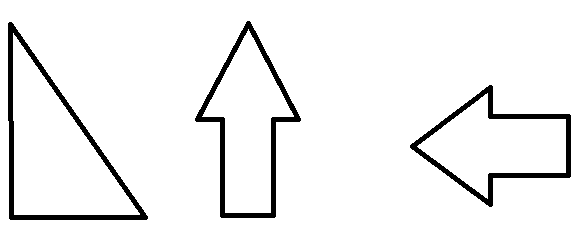
\includegraphics[scale=0.3]{mypicture.png}
\end{figure}}


% -------------------------------
% WIE
% -------------------------------

\newcommand{\useraction}{...}

\newcommand{\reaction}{...}

\newcommand{\designnotes}{...}

% -------------------------------
% WANN
% -------------------------------

%\newcommand{\simultaneously}{}
%\newcommand{\sequentially}{}

%\newcommand{\online}{}
%\newcommand{\offline}{}

%\newcommand{\private}{}
%\newcommand{\semipublic}{}
%\newcommand{\public}{}
%\newcommand{\stationary}{}
%\newcommand{\onthego}{}

%\newcommand{\leanback}{}
%\newcommand{\leanforward}{}

%\newcommand{\single}{}
%\newcommand{\collaboration}{}

%\newcommand{\smalltask}{}
%\newcommand{\repeatedtask}{}
%\newcommand{\locationbased}{}
%\newcommand{\distraction}{}
%\newcommand{\urgent}{}

\newcommand{\validcontext}{...}

\newcommand{\notvalidcontext}{...}


\newcommand{\devicetabular}{
\begin{tabular}[H]{|c|c|c|c|c|c|}
\hline 
von/nach & Smartwatch & Smartphone & Tablet & Tabletop & Screens \\ 
\hline 
Smartwatch & • & • & • & • & • \\ 
\hline 
Smartphone & • & • & • & • & •\\ 
\hline 
Tablet & • & • & • & • & •\\ 
\hline 
Tabletop & • & • & • & • & •\\ 
\hline
Screens & • & • & • & • & • \\ 
\hline 
\end{tabular} }


%\newcommand{\distanceA}{}
%\newcommand{\distanceB}{}
%\newcommand{\distanceC}{}
%\newcommand{\distanceD}{}

% -------------------------------
% WARUM
% -------------------------------

%\newcommand{\established}{}
%\newcommand{\candidate}{}
%\newcommand{\realizable}{}
%\newcommand{\futuristic}{}

\newcommand{\otherpatterns}{...}

\newcommand{\stateoftheart}{...}

%\newcommand{\designprinciples}{}

%\newcommand{\imageschemata}{}
%\newcommand{\imageschemataA}{}
%\newcommand{\imageschemataB}{}
%\newcommand{\imageschemataC}{}

%\newcommand{\realworld}{}
%\newcommand{\realworldA}{}
%\newcommand{\realworldB}{}
%\newcommand{\realworldC}{}
%\newcommand{\realworldD}{}

%\newcommand{\metaphor}{}

% -------------------------------
% TECHNISCHES
% -------------------------------

\newcommand{\technologyObjectA}{}
\newcommand{\technologyObjectB}{}
\newcommand{\technologyObjectC}{}
\newcommand{\technologyObjectD}{}
\newcommand{\technologyObjectDesc}{...}

\newcommand{\technologyCommunicationServer}{}
\newcommand{\technologyCommunicationAdhoc}{}
\newcommand{\technologyCommunicationDesc}{...}

\newcommand{\technologyOrientationAccelerometer}{}
\newcommand{\technologyOrientationGPS}{}
\newcommand{\technologyOrientationGyroskop}{}
\newcommand{\technologyOrientationAnnaeherung}{}
\newcommand{\technologyOrientationHoehe}{}
\newcommand{\technologyOrientationBeacons}{}
\newcommand{\technologyOrientationOther}{}
\newcommand{\technologyOrientationDesc}{...}

\newcommand{\prototype}{...}

% -------------------------------
% SONSTIGES
% -------------------------------

\newcommand{\authors}{...}
\newcommand{\literature}{...}
\newcommand{\figures}{...}
\newcommand{\versionhistory}{...}
\newcommand{\comments}{...}
\newcommand{\questions}{...}


% template inkludieren --------------

\begin{document}

% ------ fixes the build for all patterns where those new variables haven't been defined yet
\ifdefined\reactionSen
\else
\newcommand{\reactionSen}{tbd.}
\fi

\ifdefined\reactionRec
\else
\newcommand{\reactionRec}{tbd.}
\fi

\ifdefined\microinteractionstabular
\else
\newcommand{\microinteractionstabular}{tbd.}
\fi

\ifdefined\animations
\else
\newcommand{\animations}{tbd.}
\fi

\ifdefined\requiredTechnologies
\else
\newcommand{\requiredTechnologies}{tbd.}
\fi

\ifdefined\implementation
\else
\newcommand{\implementation}{tbd.}
\fi

\maketitle

%----------------------------
% CATEGORY ICON
%----------------------------
\begin{textblock}{2}[0,0](8, -3)
\ifthenelse{\equal{\category}{give}}{\newcommand{\icon}{icon_give.png}}{}
\ifthenelse{\equal{\category}{take}}{\newcommand{\icon}{icon_take.png}}{}
\ifthenelse{\equal{\category}{connect}}{\newcommand{\icon}{icon_connect.png}}{}
\ifthenelse{\equal{\category}{extend}}{\newcommand{\icon}{icon_extend.png}}{}
\ifthenelse{\equal{\category}{exchange}}{\newcommand{\icon}{icon_exchange.png}}{}	
\includegraphics[scale=0.5]{\icon}
\end{textblock}

% -------------------------------
% WAS
% -------------------------------
\section*{Was}

\subsection*{Problem}
\desc

\subsection*{Lösung}
\solution

\subsection*{Grafische Darstellung}
\begin{figure}[H]
\IfFileExists{\jobname_graphical_description.png}{\includegraphics[width=\textwidth]{\grafischedarstellung}}{}
\end{figure}

\subsection*{Kategorie}
\ifthenelse{\equal{\category}{give}}{$\boxtimes$}{$\Box$} Give   |   
\ifthenelse{\equal{\category}{take}}{$\boxtimes$}{$\Box$} Take   |   
\ifthenelse{\equal{\category}{exchange}}{$\boxtimes$}{$\Box$} Exchange   |   
\ifthenelse{\equal{\category}{extend}}{$\boxtimes$}{$\Box$} Extend   |   
\ifthenelse{\equal{\category}{connect}}{$\boxtimes$}{$\Box$} Connect

% -------------------------------
% WIE
% -------------------------------
\newpage
\section*{Wie}

\subsection*{Aktion des \sen s}
\useraction

\subsection*{Reaktionen des \sendev s}
\reactionSen

\subsection*{Reaktionen des \recdev s}
\reactionRec

\subsection*{Übersicht über die Microinteractions}
\microinteractionstabular

\subsubsection*{Animationen}
\animations

\subsection*{Hinweise zur Gestaltung der Interaktion}
\designnotes

% -------------------------------
% WANN
% -------------------------------

\section*{Wann}

\subsection*{Geeigneter Nutzungskontext}
\validcontext

\subsubsection*{Zeit}
\checkbox{\simultaneously} gleichzeitige Nutzung der beteiligten Geräte \\
\checkbox{\sequentially} sequentielle Nutzung der beteiligten Geräte

\subsubsection*{Ort}
\checkbox{\private} privat \\
\checkbox{\semipublic} halb-öffentlich \\
\checkbox{\public} öffentlich \\
\checkbox{\stationary} stationär \\
\checkbox{\onthego} unterwegs 

\subsubsection*{Körperhaltung der Benutzer}
\checkbox{\leanback} Lean-Back \\
\checkbox{\leanforward} Lean-Forward 

\subsubsection*{Teilnehmer}
\checkbox{\single} Einzelnutzer \\
\checkbox{\collaboration} Kollaboration

\subsubsection*{Anordnung zwischen Sender und Empfänger}
\checkbox{\facetoface} Face-To-Face \\
\checkbox{\sidetoside} Side-To-Side

\subsection*{Abzuratender Nutzungskontext}
\notvalidcontext

\subsection*{Geräteklassen}
\devicetabular


% -------------------------------
% WARUM
% -------------------------------

\section*{Warum}
\checkbox{\established} Bewährtes Interaction Pattern \\
\checkbox{\candidate} Interaction Pattern Kandidat: 
\checkbox{\realizable} realisierbar oder
\checkbox{\futuristic} futuristisch

\subsection*{Verwandte Patterns}
\otherpatterns

\subsection*{State of the Art}
\stateoftheart

\subsection*{Checkliste: Entspricht die Interaktion der Definiton einer "Blended Interaction"?}
\checkbox{\designprinciples} Werden die Designprinzipien berücksichtigt?
\begin{itemize}
\item[-] Die Interaktion greift eine Metapher aus der physikalischen Welt auf.
\item[-] Die Interaktion kann in einer Kollaboration ausgeführt werden.
\item[-] Die Interaktion unterstützt einen Workflow/eine Aufgabe.
\item[-] Die Interaktion findet in einer physikalischen Umgebung statt.
\end{itemize} 

\checkbox{\imageschemata} Image Schema/ta liegen zu Grunde.
\begin{itemize}
\item[-] \checkbox{\imageSchemaContainer} Container
\item[-] \checkbox{\imageSchemaInOut} In-Out
\item[-] \checkbox{\imageSchemaPath} Path
\item[-] \checkbox{\imageSchemaSourcePathGoal} Source-Path-Goal
\item[-] \checkbox{\imageSchemaUpDown} Up-Down
\item[-] \checkbox{\imageSchemaLeftRight} Left-Right
\item[-] \checkbox{\imageSchemaNearFar} Near-Far
\item[-] \checkbox{\imageSchemaPartWhole} Part-Whole
\end{itemize}

\checkbox{\realworld} Die real-weltlichen Kenntnisse des Menschen werden berücksichtigt.
\begin{itemize}
\item[-] \checkbox{\realworldNaivePhysic} Naive Physik
\item[-] \checkbox{\realworldBodyAwareness} Body Awareness and Skills
\item[-] \checkbox{\realworldEnvironmentAwareness} Environmental Awareness and Skills
\item[-] \checkbox{\realworldSocialAwareness} Social Awareness and Skills
\end{itemize}

\checkbox{\metaphor} Es ist eine natürliche Interaktion. Metapher/Assoziation: \metaphordesc

% -------------------------------
% TECHNISCHES
% -------------------------------

\section*{Technisches}

\subsection*{Benötigte Technologien}
\requiredTechnologies

\subsection*{Implementierungshinweise}
\implementation

% -------------------------------
% SONSTIGES
% -------------------------------

\section*{Sonstiges}

\subsection*{Autor/en}
\authors

\subsection*{Versionshistorie}
Erstelldatum: \dateofcreation \\
Letzte Änderung am: \versionhistory

\subsection*{Kommentare}
\comments

\subsection*{Offene Fragen}
\questions

\listoffigures

\printbibliography

\clearpage

\printglossaries

\end{document}